\documentclass[a4paper,11pt]{article}
\usepackage[utf8]{inputenc}
\usepackage{titling}
\usepackage[a4paper,margin=0.75in]{geometry} % Adjust the margins here
\usepackage{amsmath,amssymb,amsfonts}
\usepackage{algorithmic}
\usepackage{graphicx}
\usepackage{textcomp}
\usepackage{comment}
\usepackage{xcolor}
\usepackage{enumitem}
\usepackage{tcolorbox}
\usepackage{listings}
\tcbuselibrary{listings,skins}  

\usepackage{changepage}

\usepackage{caption}
\usepackage{draftwatermark}
\usepackage{environ}

\usepackage{lmodern} % Optional: Use a scalable font family
\usepackage{scalefnt} % Optional: Allow smooth font scaling

\usepackage{siunitx} % ohm symbol

\usepackage{fancyvrb}     % for the Verbatim environment
% Customize watermark
\SetWatermarkText{\scalefont{1.5}GOWDA} % Use scalefont for scaling
\SetWatermarkScale{.2} % Adjust scale to avoid very large fonts
\SetWatermarkColor[gray]{0.7} % Light gray (80% white)
\SetWatermarkAngle{30}
%\SetWatermarkHorCenter{8cm} % Move right by 3 cm
%\SetWatermarkVerCenter{18cm} % Move up by 12 cm




\newtcblisting{codebox}[2][]{%
  colback=blue!10,           
  colframe=black,                       
  boxrule=1pt,               
  title={#2},                
  listing only,              
  listing engine=listings,   
  listing options={%
    language=Python,
    upquote = true,
    basicstyle=\ttfamily\small,
    breaklines=true,
    showstringspaces=false,
    frame=none,
    xleftmargin=0pt,
    xrightmargin=0pt,
    aboveskip=0pt,
    belowskip=0pt,
    #1
  },
}

\newtcblisting{outputs}[1][]{%
  colback=green!10,
  colframe=black,
  boxrule=1pt,
  title={Output:},
  listing only,
  listing engine=listings,
  listing options={%
    language=Python,
    upquote = true,
    basicstyle=\ttfamily\small,
    commentstyle=\ttfamily\small,
    breaklines=true,
    showstringspaces=false,
    frame=none,
    xleftmargin=0pt, xrightmargin=0pt, aboveskip=0pt, belowskip=0pt,
    columns=fullflexible,
    #1
  },
}

\newtcblisting{syntax}[1][]{%  ← only one optional argument now
  colback=red!10,
  colframe=black,
  boxrule=1pt,
  title={Syntax:},         % ← fixed, constant title
  listing only,
  listing engine=listings,
  listing options={%
    language=Python,
    upquote=true,
    basicstyle=\ttfamily\small,
    breaklines=true,
    showstringspaces=false,
    frame=none,
    xleftmargin=0pt,
    xrightmargin=0pt,
    aboveskip=0pt,
    belowskip=0pt,
    #1                            % any per-box overrides
  },
}


\title{Introduction to Programming \\ Lab: Understanding Variables and Data Types}
\author{Vikas Thammanna Gowda}
\date{07/15/2025}

\lstset{
    language=Python,
    basicstyle=\ttfamily\small,
    keywordstyle=\bfseries,
    showstringspaces=false,
    breaklines=true,
    frame=none,
    xleftmargin=5pt,
    xrightmargin=5pt,
    aboveskip=10pt,
    belowskip=5pt,
    captionpos=b
}
\begin{document}
\maketitle

\noindent \textbf{Name: \_\_\_\_\_\_\_\_\_\_\_\_\_\_\_\_\_\_\_\_\_\_\_\_\_\_\_\_\_\_\_\_\_\_\_\_\_\_\_\_\_\_\_\_\_\_\_}
\section*{Introduction}
In this lab, you will connect a DHT22 digital temperature sensor and a 20 $\times$ 4 LCD display 
to a Raspberry Pi to create a simple digital thermometer. 

The lab is split into two parts: 
\begin{itemize}
\item \textbf{Part 1:} You will be provided with the \textit{complete code, circuit diagram, setup, 
and wiring instructions}, along with a \textit{brief in-class demonstration}. In this part, 
you will use the DHT22 sensor to measure the ambient temperature in 
degrees Celsius, and humidity as a percentage of relative humidity and display the readings on the LCD. 

\item \textbf{Part 2:} A collaborative activity to extend the code to display the 
temperature in Fahrenheit and Kelvin as well.

\end{itemize} 

\subsection*{Learning Objectives}
\begin{itemize}
    \item Understand how to read sensor data (temperature) from the DHT22 using Raspberry Pi.

\item Use variables to store sensor values and apply arithmetic operators for unit conversion (Celsius to Fahrenheit and Kelvin).

\item Distinguish and convert between data types (e.g., float to string).

\item Format and display multi-line text on a 20 $\times$ 4 LCD.

\item Gain experience integrating hardware (sensor + LCD) with Python code.

\end{itemize}

\subsection*{Required Components:}
\begin{itemize}
    \item Raspberry Pi (any model with 40 GPIO pins) with Raspbian/Raspberry Pi OS installed. 
\item Breadboard and jumper wires.
\item DHT22 temperature/humidity sensor with a 10 k$\Omega$ resistor for the required pull-up between its data pin and 3.3V
\item 20x4 Character LCD.
\end{itemize}


\newpage
\section*{Part 1: Reading Celsius Temperature and Humidity}
In the first part of the lab, we will run a Python program on the Raspberry Pi to 
read the temperature from the DHT22 and display it on the LCD in Celsius. 
This will introduce how the program uses variables and their data types to 
store the sensor data, and how it outputs it to the display.


\subsection*{Illustration}

Follow these steps to assemble the LED circuit. \textbf{Make sure your Raspberry Pi 
is shut down or powered off while wiring the circuit to avoid any accidental 
short circuits or damage.}

\subsubsection*{DHT22 Sensor Wiring:}
The DHT22 has three pins: VCC (power), Data out, and GND. 
We will use a 10 k$\Omega$  resistor as a pull-up on the data line (connecting data to VCC) 
to ensure reliable communication. Wire the DHT22 to the Raspberry Pi as follows:

    \begin{figure}[h] % 'h' places the figure approximately here
        \centering
        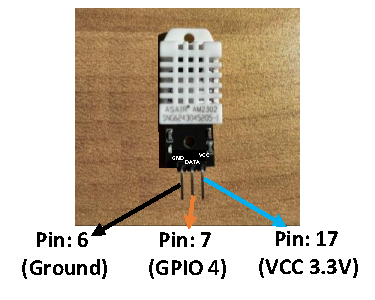
\includegraphics[width=.65\textwidth]{fig1.pdf} % Change size as needed
        \caption{DHT22 Sensor connection to Raspberry Pi's GPIO pins}
        \label{fig:runtime}
    \end{figure}

\begin{enumerate}
  \item Place a 10 k$\Omega$  resistor between the DHT22's VCC pin (pin 1) and Data pin (pin 2) on the breadboard.
This resistor acts as a pull-up, tying the data line to 3.3V when idle.
(If you had a DHT22 module on a breakout board, this resistor would typically be built-in.)
\item Connect DHT22 pin 3 (VCC) to the Raspberry Pi's 3.3V power pin (e.g. physical pin 17 on the Pi)
\item Connect DHT22 pin 2 (Data) to a Raspberry Pi GPIO input pin. In our example, we'll use GPIO4 (physical pin 7) which is a common default for DHT sensors.
\item Connect DHT22 pin 1 (GND) to a ground pin on the Raspberry Pi (physical pin 6 or any other GND)

\end{enumerate}

\noindent \textbf{Note: The DHT22 should be powered at 3.3V (not 5V) when used with the Pi, to keep the data signal at Pi-safe voltage levels. Also, the sensor cannot be read more often than once every 2 seconds (approx.), as it needs time to take a measurement.}


\subsubsection*{LCD Display Wiring:}
For the 20×4 character LCD, we assume it has an I²C interface adapter attached. 
This adapter greatly simplifies the wiring by using only four connections.

\begin{figure}[h] % 'h' places the figure approximately here
    \centering
    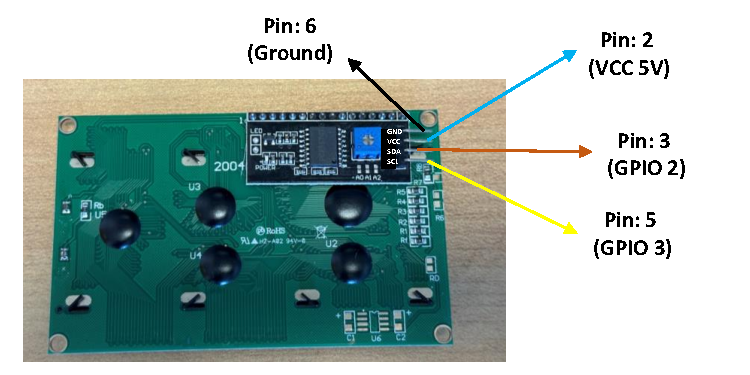
\includegraphics[width=.85\textwidth]{fig3.pdf} % Change size as needed
    \caption{LCD connection to Raspberry Pi's GPIO pins.}
    \label{fig:LCD}
\end{figure}

\begin{enumerate}
    \item Connect the LCD module's VCC pin to the Pi's 5V power (physical pin 2 or 4), 
    and the LCD GND to a Pi GND pin 6.

    \item Connect the LCD’s SDA pin to the Pi’s SDA line. On Raspberry Pi, SDA corresponds to GPIO 2 (physical pin 3)

    \item Connect the LCD's SCL pin to the Pi's SCL line, which is GPIO 3 (physical pin 5).

\end{enumerate}

\begin{figure}[h] % 'h' places the figure approximately here
    \centering
    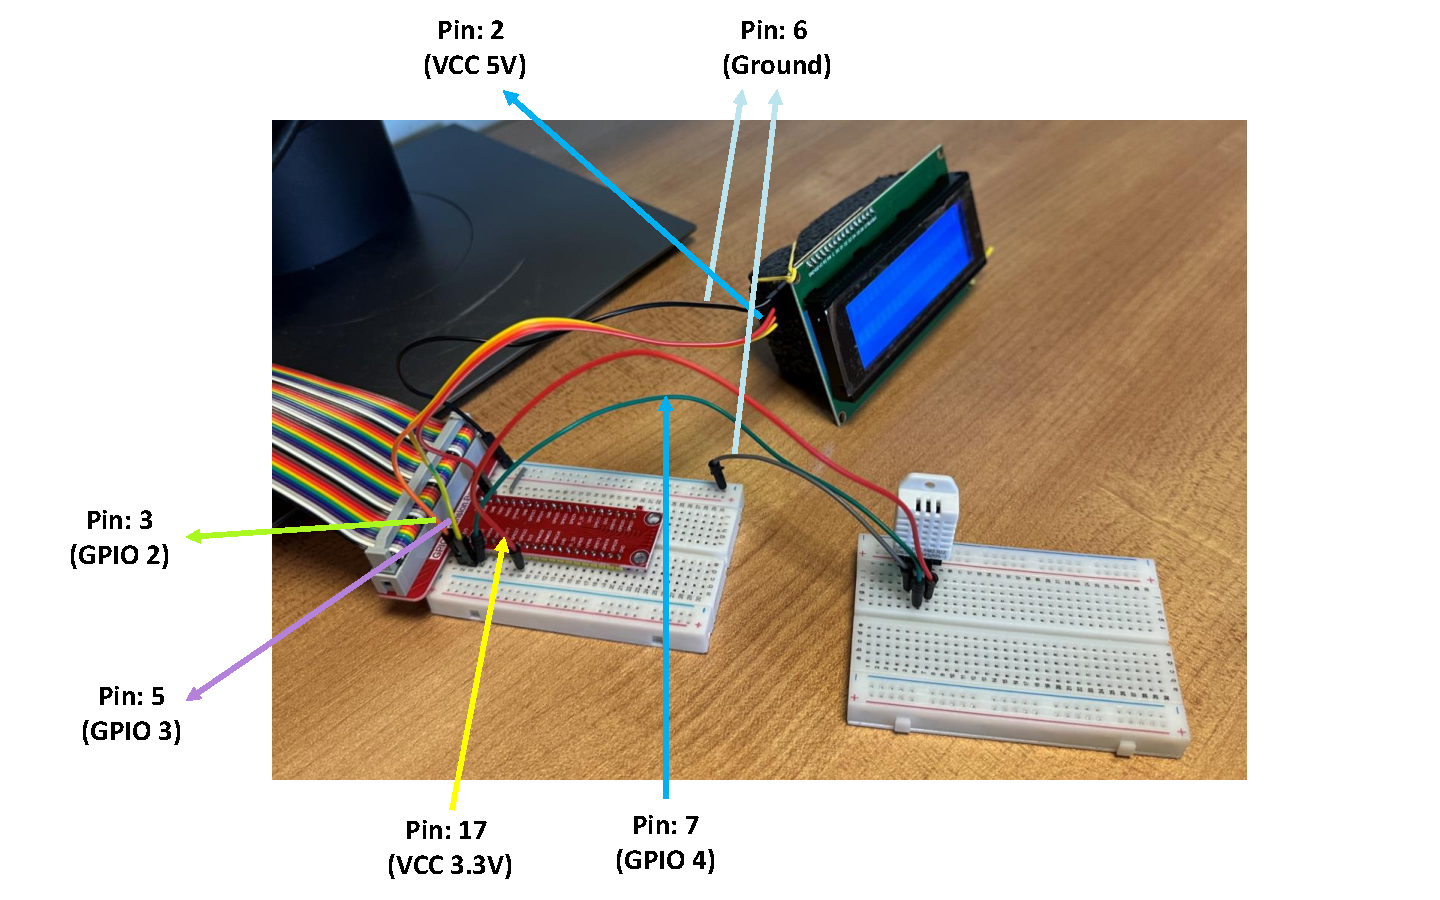
\includegraphics[width=.85\textwidth]{fig2.pdf} % Change size as needed
    \caption{Wiring set-up.}
    \label{fig:runtime1}
\end{figure}

\newpage
\subsection*{Run and Observe}
It’s time to test the circuit and code. Make sure your 
Raspberry Pi is powered on and the circuit is connected as described. 
Run the privided Python script.

\subsection*{Record your observations:}
\begin{table}[ht]
  \centering
  \renewcommand{\arraystretch}{1.5}
  \begin{tabular}{|p{1cm}|c|c|}
    \hline
    \textbf{No.} & \textbf{Temperature} & \textbf{Humidity} \\ \hline
     &  &  \\ \hline
     &  &  \\ \hline
     &  &  \\ \hline
     &  &  \\ \hline
     &  &  \\ \hline
     &  &  \\ \hline
     &  &  \\ \hline
     &  &  \\ \hline
     &  &  \\ \hline
     &  &  \\ \hline
  \end{tabular}
  \caption{Temperature in \(^\circ\text{C}\) and Humidity Reading}
  \label{tab:empty-3x10}
\end{table}

\newpage
\section*{Part 2: Converting Temperature to Fahrenheit and Kelvin }
After getting the Celsius display working, the next step (and main goal of this lab exercise) 
is to modify the code to also display the temperature in Fahrenheit and Kelvin. 
This will involve using arithmetic operators in our code to convert the values, 
and handling additional variables for the new values. This is where we practice 
using operators to compute new results from existing data.

\subsection*{Formulas for Conversion} 
The formulas to convert temperature scales are well known:

\begin{itemize}
  \item \textbf{Celsius to Fahrenheit:} 
  $$F = \left( \frac{9}{5} \times C \right) + 32$$

  \item \textbf{Celsius to Kelvin:} 
  $$K = C + 273.15$$

\end{itemize}

So, for example, if the sensor reads \(25.0^\circ\text{C}\), then:

$$
^\circ\text{F} = 25.0 \times \frac{9}{5} + 32 = 77.0^\circ\text{F}
$$

$$
K = 25.0 + 273.15 = 298.15\ \text{K}
$$

\subsection*{Record your observations:}

\begin{table}[ht]
  \centering
  % increase row height by a factor of 1.5 (optional)
  \renewcommand{\arraystretch}{1.5}
  \begin{tabular}{|p{1cm}|p{3cm}|p{3cm}|p{3cm}|}
    \hline
    \textbf{No.} & \textbf{\(^\circ\text{C}\)} & \textbf{\(^\circ\text{F}\)} & \textbf{\(^\circ\text{K}\)} \\ \hline
    1 & 25.0 & 77.0 & 298.15 \\ \hline
     &  &  &  \\ \hline
     &  &  &  \\ \hline
     &  &  &  \\ \hline
     &  &  &  \\ \hline
     &  &  &  \\ \hline
     &  &  &  \\ \hline
     &  &  &  \\ \hline
     &  &  &  \\ \hline
     &  &  &  \\ \hline
  \end{tabular}
  \caption{Temperature reading}
  \label{tab:4x10}
\end{table}


\newpage
\section*{Reflection and Analysis}
\begin{enumerate}
    \item How did using variables help in organizing your code and making it easier to modify?

\item Was it clear when and why you needed to convert between data types (e.g., float to string for display)?

\item Did your displayed values match your expectations (e.g., were the conversions accurate)? How did you verify this?

\item How confident do you feel now about applying basic arithmetic operations in code?

\item What was the most challenging part of combining hardware readings with software display?

    \item \textbf{Further extension:} Discuss how his project can be extended.

\end{enumerate}

\end{document}